\chapter{ یادگیری تقویتی}
\section{مقدمه}
به طور عمومی، یادگیری ماشین به دسته‌ای از الگوریتم‌ها و روش‌های محاسباتی گفته می‌شود که به ماشین‌ها امکان یادگیری از داده‌ها و تجربه‌های خود را می‌دهند.
یادگیری ماشین به دو دسته‌ی اصلی تقسیم می‌شود: یادگیری نظارت‌شده\LTRfootnote{Supervised Learning}
 و یادگیری بدون نظارت\LTRfootnote{Unsupervised Learning}.
در یادگیری نظارت‌شده، مدل به کمک داده‌های برچسب‌خورده آموزش داده می‌شود و سپس برای پیش‌بینی خروجی‌های جدید از این مدل استفاده می‌شود.
در یادگیری بدون نظارت، مدل بدون داده‌های برچسب‌خورده آموزش داده می‌شود و باید خودش مفاهیم و الگوهای موجود در داده‌ها را کشف کند.
یادگیری تقویتی در این دو دسته قرار نمی‌گیرد و به عنوان یک دسته جداگانه در نظر گرفته می‌شود.

یادگیری تقویتی یک روش یادگیری ماشین است که به عامل اجازه می‌دهد تا رفتار بهینه را از طریق تعامل و آزمون و خطا با محیط یاد بگیرد.
در این روش، عامل مشاهدات خود را از محیط (به کمک حسگر)
دریافت کرده،
و بر اساس آن تصمیم خود را اخذ می‌کند.
پس از انجام هر عمل، محیط به عامل پاداشی می‌دهد که نشان‌دهنده‌ی عملکرد عامل در آن حالت است.
هدف این است که عامل مجموع پاداش‌های دریافتی خود را بیشینه کند؛ که در صورت صحیح بودن تعریف سیگنال پاداش، معمولا به معنای رسیدن به هدف مطلوب است.

یادگیری تقویتی با سایر رویکرد‌های یادگیری ماشین مانند یادگیری نظارت‌شده و یادگیری بدون نظارت تفاوت‌های زیادی دارد، 
و معمولا بر مسائلی به کار می‌رود که تمرکز بر تصمیم‌گیری یا پیدا کردن سیاست بهینه بدون نیاز به داده‌های برچسب‌خورده است.
در عوض، عامل با اکتشاف و بهره‌برداری ابتدا انتقالات بین حالت‌ها و پاداش‌های مرتبط با آن‌ها را یاد می‌گیرد، و سپس سیاستی را یاد می‌گیرد که مجموع پاداش‌ها را بیشینه کند.


\section{اصول یادگیری تقویتی}
\subsection{عامل، محیط، حالت، عمل و پاداش}
در یادگیری تقویتی، عامل\LTRfootnote{Agent}
 تصمیم‌گیرنده برای رسیدن به هدف خود با محیط\LTRfootnote{Environment}
  تعامل دارد.
محیط معمولا به صورت مجموعه‌ای از حالت‌ها\LTRfootnote{State}
  و عمل‌هایی\LTRfootnote{Action}
    که عامل می‌تواند انجام دهد مدل می‌شود.
در هر گام، عامل مشاهده‌ای از حالت محیط را دریافت می‌کند و بر اساس آن تصمیمی اتخاذ می‌کند.
پس از انجام عمل، محیط به عامل پاداش\LTRfootnote{Reward}
  می‌دهد که نشان‌دهنده‌ی عملکرد عامل در آن حالت است.

\begin{figure}[H]
    \centering
    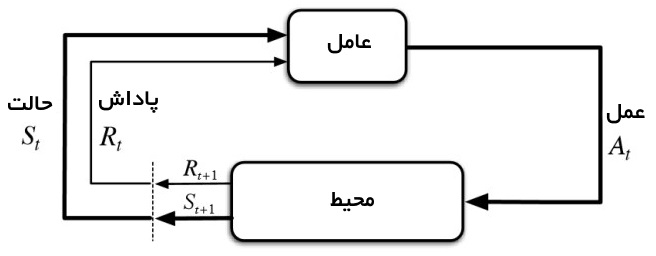
\includegraphics[width=0.75\textwidth]{images/agent_env.jpg}
    \caption{تعامل عامل و محیط}\label{fig:agent_env}

\end{figure}
% explain episodes here
در اکثر مواقع، یادگیری تقویتی در مسائلی استفاده می‌شود که بتوان آن را به دنباله‌ای از گام‌ها تقسیم کرد که قطعا به یک حالت پایانی می‌رسد.
 هر یک از این دنباله‌ها را قسمت\LTRfootnote{Episode}
  می‌نامند.
\subsection{فرایند تصمیم‌گیری مارکوف}
فرایند تصمیم‌گیری مارکوف\LTRfootnote{Markov Decision Process (MDP)}
  مدلی است برای تصمیم‌گیری در محیط‌هایی که به صورت مارکوف هستند.
  محیط‌های دارای خاصیت مارکوف، محیط‌هایی هستند که حالت بعدی به صورت کامل به حالت فعلی و عمل انجام شده وابسته است.


  یک فرایند تصمیم‌گیری مارکوف، چهارتایی 
  $(S, A, P, R)$
  است که در آن:
  \begin{itemize}
      \item $S$ مجموعه‌ی تمام حالت‌های ممکن محیط است.
      \item $A$ مجموعه‌ی تمام عمل‌های ممکن است.
      \item $P$ تابع انتقال\LTRfootnote{Transition Function}
      است که به ازای هر حالت و عمل، توزیع احتمال حالت بعدی را مشخص می‌کند.
      \item $R$ تابع پاداش\LTRfootnote{Reward Function}
      است که به ازای هر حالت و عمل، پاداش مورد انتظار را مشخص می‌کند.
      \item نرخ تخفیف $\gamma$ نیز معمولا به عنوان یک پارامتر دیگر در نظر گرفته می‌شود که نشان‌دهنده‌ی اهمیت پاداش‌های آینده نسبت به پاداش‌های فعلی است.
  \end{itemize}
همانطور که گفته شد، در هر گام عامل با اخذ تصمیم خود، محیط را به حالت جدیدی می‌برد و پاداشی دریافت می‌کند.
به مجموع کل پاداش‌هایی که عامل در یک قسمت دریافت می‌کند، خروجی\LTRfootnote{Return}
 گفته می‌شود.
 \begin{equation}\label{eq:return}
     G_t = R_{t+1} + \gamma \times R_{t+2} + \gamma^2 \times R_{t+3} + \cdots = \sum_{k=0}^\infty \gamma^k \times R_{t+k+1}
 \end{equation}
\subsection{سیاست، تابع ارزش، و تابع ارزش عمل}
سیاست\LTRfootnote{Policy}
یک تابع از حالت‌ها به عمل‌ها است که نشان‌دهنده‌ی رفتار عامل در هر حالت محیط است.
در واقع مسئله یادگیری تقویتی را می‌توان به «یافتن سیاستی که مجموع پاداش‌ها را بیشینه می‌کند» تعبیر کرد.
\begin{equation}\label{eq:policy}
    \pi(a|s) = \mathbb{P}\{A_t = a | S_t = s\}
\end{equation}

تابع ارزش\LTRfootnote{Value Function} $V(s)$
یک تابع از حالت‌ها است که نشان‌دهنده‌ی میزان پاداش مورد انتظار از یک حالت تا به انتهای قسمت است.
\begin{equation}\label{eq:value_function}
    v_\pi(s) = \mathbb{E}_\pi\{G_t | S_t = s\} = \sum_{a \in A}\pi(a|s)\times\{R_s^a + \gamma \times \sum_{s' \in S}p(s'|s,a)\times v_\pi(s')\}
\end{equation}
تابع ارزش عمل\LTRfootnote{Action Value Function} $Q(s, a)$
نیز مشابه تابع ارزش است؛ با این تفاوت که به جای حالت، از یک حالت و یک عمل مشخص محاسبه می‌شود. رایج است که به این تابع، تابع کیو گفته شود.
\begin{equation}\label{eq:q_function}
    q_\pi(s,a) = \mathbb{E}_\pi\{G_t | S_t = s, A_t = a\} = R_s^a + \gamma \times \sum_{s' \in S}p(s'|s,a)\times v_\pi(s')
\end{equation}
به این معادلات، که از کلیدی‌ترین روابط در یادگیری تقویتی هستند، معادله بلمن\LTRfootnote{Bellman Equation} گفته می‌شود.
\section{الگوریتم‌های پایه یادگیری تقویتی}
\subsection{برنامه‌نویسی پویا}
همان‌طور که در معادله \ref{eq:value_function} مشخص است، می‌توان تابع ارزش را به صورت بازگشتی محاسبه کرد.
این روش برنامه‌نویسی پویا\LTRfootnote{Dynamic Programming}
نام دارد.
\subsubsection{یادگیری به کمک تکرار ارزش}
در روش تکرار ارزش\LTRfootnote{Value Iteration}،
 ابتدا تابع ارزش را به صورت تصادفی مقداردهی می‌کنیم و سپس آن را به صورت بازگشتی به‌روز‌رسانی می‌کنیم.
قابل اثبات است که این روش به تابع ارزش بهینه همگرا می‌شود\cite{howard1960dynamic}.
به صورت شهودی هم می‌توان دید که ارزش از سمت حالت‌های پایانی به سمت حالت‌های ابتدایی به‌روز‌رسانی می‌شود.
\subsubsection{یادگیری به کمک تکرار سیاست}
در روش تکرار سیاست\LTRfootnote{Policy Iteration}،
ابتدا سیاست را به صورت تصادفی مقداردهی می‌کنیم و سپس تابع ارزش را برای آن محاسبه می‌کنیم.
سپس سیاست را به صورتی تغییر می‌دهیم که در هر گام عامل به حالت بعدی ممکن با بیشترین ارزش برود.
این فرآیند را تا زمانی که سیاست تغییر نکند ادامه می‌دهیم.
قابل اثبات است که این روش به سیاست بهینه همگرا می‌شود.

در عمل، با توجه به اینکه معمولا به تابع انتقال دسترسی نداریم، نمی‌توانیم از روش‌های برنامه‌نویسی پویا به صورت مستقیم استفاده کنیم.
در واقع نیاز به راه حل‌های مستقل از مدل داریم که به کمک نمونه‌برداری\LTRfootnote{Sampling}
 و کاوش\LTRfootnote{Exploration}
 محیط، سیاست بهینه را یاد بگیرند.

\subsection{یادگیری به کمک نمونه‌برداری مونته کارلو}
در روش‌های یادگیری به کمک نمونه‌برداری مونته کارلو\LTRfootnote{Monte Carlo Sampling}،
به جای استفاده از مدل، از نمونه‌برداری برای تخمین ارزش استفاده می‌شود\cite{barto2021reinforcement}.
کافی‌ست ابتدا یک قسمت را به طور کامل اجرا کنیم، و سپس ارزش هر حالت را، به سمت خروجی قسمت، به‌روز‌رسانی کنیم:
\begin{equation}\label{eq:mc_q_function}
    Q(s_t, a_t) = Q(s_t, a_t) + \alpha \times (G_t - Q(s_t, a_t))
\end{equation}
که در این فرمول، $\alpha$
نرخ یادگیری\LTRfootnote{Learning Rate} است.

لازم به ذکر است که در حین اجرای قسمت، از سیاست اپسیلون-حریصانه\LTRfootnote{$\epsilon$-greedy} استفاده می‌شود.
در این سیاست، با احتمال $\epsilon$ عملی تصادفی انجام می‌شود و با احتمال $1-\epsilon$ عملی که بیشترین ارزش را دارد انجام می‌شود.
دلیل استفاده از این سیاست، نیاز به کاوش محیط و جلوگیری از گیر کردن در حالت‌های محلی است.

از معایب این روش، می‌توان به نیاز به اجرای کامل قسمت‌ها و نیاز به زمان برای یادگیری اشاره کرد. به همین دلیل، این روش برای مسائلی که قسمت‌های طولانی دارند، مناسب نیست.
از مشکلات دیگر این روش، عدم استفاده از ویژگی مارکوف محیط است.
\subsection{یادگیری به کمک تفاوت زمانی}
همان‌طور که گفته شد، استفاده از یادگیری مونته‌کارلو باعث می‌شود که عامل در حین انجام قسمت، از تجربه‌ی قبلی خود استفاده نکند
و به‌روز‌رسانی ارزش‌ها فقط پس از اتمام قسمت انجام شود. به این روش، یادگیری برون‌خط\LTRfootnote{Offline Learning} گفته می‌شود.
در روش یادگیری به کمک تفاوت زمانی\LTRfootnote{Temporal Difference Learning}\cite{sutton1988learning}،
عامل در حین انجام قسمت، از تجربه‌ی خود استفاده می‌کند و ارزش‌ها را به صورت برخط\LTRfootnote{Online}
 به‌روز‌رسانی می‌کند.
در واقع به کمک معادله بلمن، مقادیر کیو به سمت مقدار کیو بعدی به‌روز‌رسانی می‌شوند.

پیاده‌سازی این دو الگوریتم، به دو روش دید رو به جلو و دید رو به عقب انجام می‌شود.
در حالت دید رو به جلو، مشابه با یادگیری مونته کارلو، پس از رسیدن به پایان قسمت، ارزش‌ها به‌روز‌رسانی می‌شوند.
در حالت دید رو به عقب، ارزش‌ها به صورت برخط به‌روز‌رسانی می‌شوند. به این صورت که پس از دریافت یک پاداش، عامل مقادیر کیو $n$ حالت‌ قبلی خود را به‌روز‌رسانی می‌کند.
\subsubsection{تی‌دی صفر}
در ساده‌ترین حالت، عامل در حین انجام عمل، با دیدن یک گام در آینده یا گذشته، ارزش عمل فعلی را به‌روز‌رسانی می‌کند.
به این روش تی‌دی صفر\LTRfootnote{TD(0)} گفته می‌شود.
\begin{equation}\label{eq:td_zero_q_function}
    Q(s_t, a_t) = Q(s_t, a_t) + \alpha \times (R_{t+1} + \gamma \times Q(s_{t+1}, a_{t+1}) - Q(s_t, a_t))
\end{equation}
در واقع، به کمک رابطه بلمن
(که فرم ارزش عمل آن در رابطه  \ref{eq:q_function} دیده می‌شود)
میزان صحیح بودن ارزش عمل فعلی، با ارزش عمل بعدی و پاداش فعلی مقایسه می‌شود و ارزش عمل فعلی به‌روز‌رسانی می‌شود.
\subsubsection{ تی‌دی لامبدا رو به جلو}
در روش تی‌دی $\lambda$\LTRfootnote{TD($\lambda$)}،
با دید رو به جلو
به جای استفاده از یک گام در آینده ، از یک ترکیب خطی از پاداش‌ها و بازگشت چندین گام استفاده می‌شود.
به این ترکیب خطی، $\lambda$-بازگشت\LTRfootnote{$\lambda$-return} گفته می‌شود.
\begin{equation}\label{eq:td_lambda_q_function}
    Q(s_t, a_t) = Q(s_t, a_t) + \alpha \times (G_t^\lambda - Q(s_t, a_t))
\end{equation}
که در این رابطه، $G_t^\lambda$
به صورت زیر محاسبه می‌شود:
\begin{equation}\label{eq:td_lambda_return}
    G_t^\lambda = (1-\lambda)\times\sum_{n=1}^\infty \lambda^{n-1} \times G_t^{(n)}
\end{equation}
که در آن $G_t^{(n)}$، 
مقدار بازگشتی بعد از $n$ گام است،
و $\lambda$
یک پارامتر بین صفر و یک است که نشان‌دهنده‌ی اهمیت پاداش‌های آینده نسبت به پاداش‌های فعلی است.
می‌توان میزان اهمیت پاداش‌های را به ازای مقادیر مختلف $\lambda$ مشاهده کرد.
\begin{figure}[H]
    \centering
    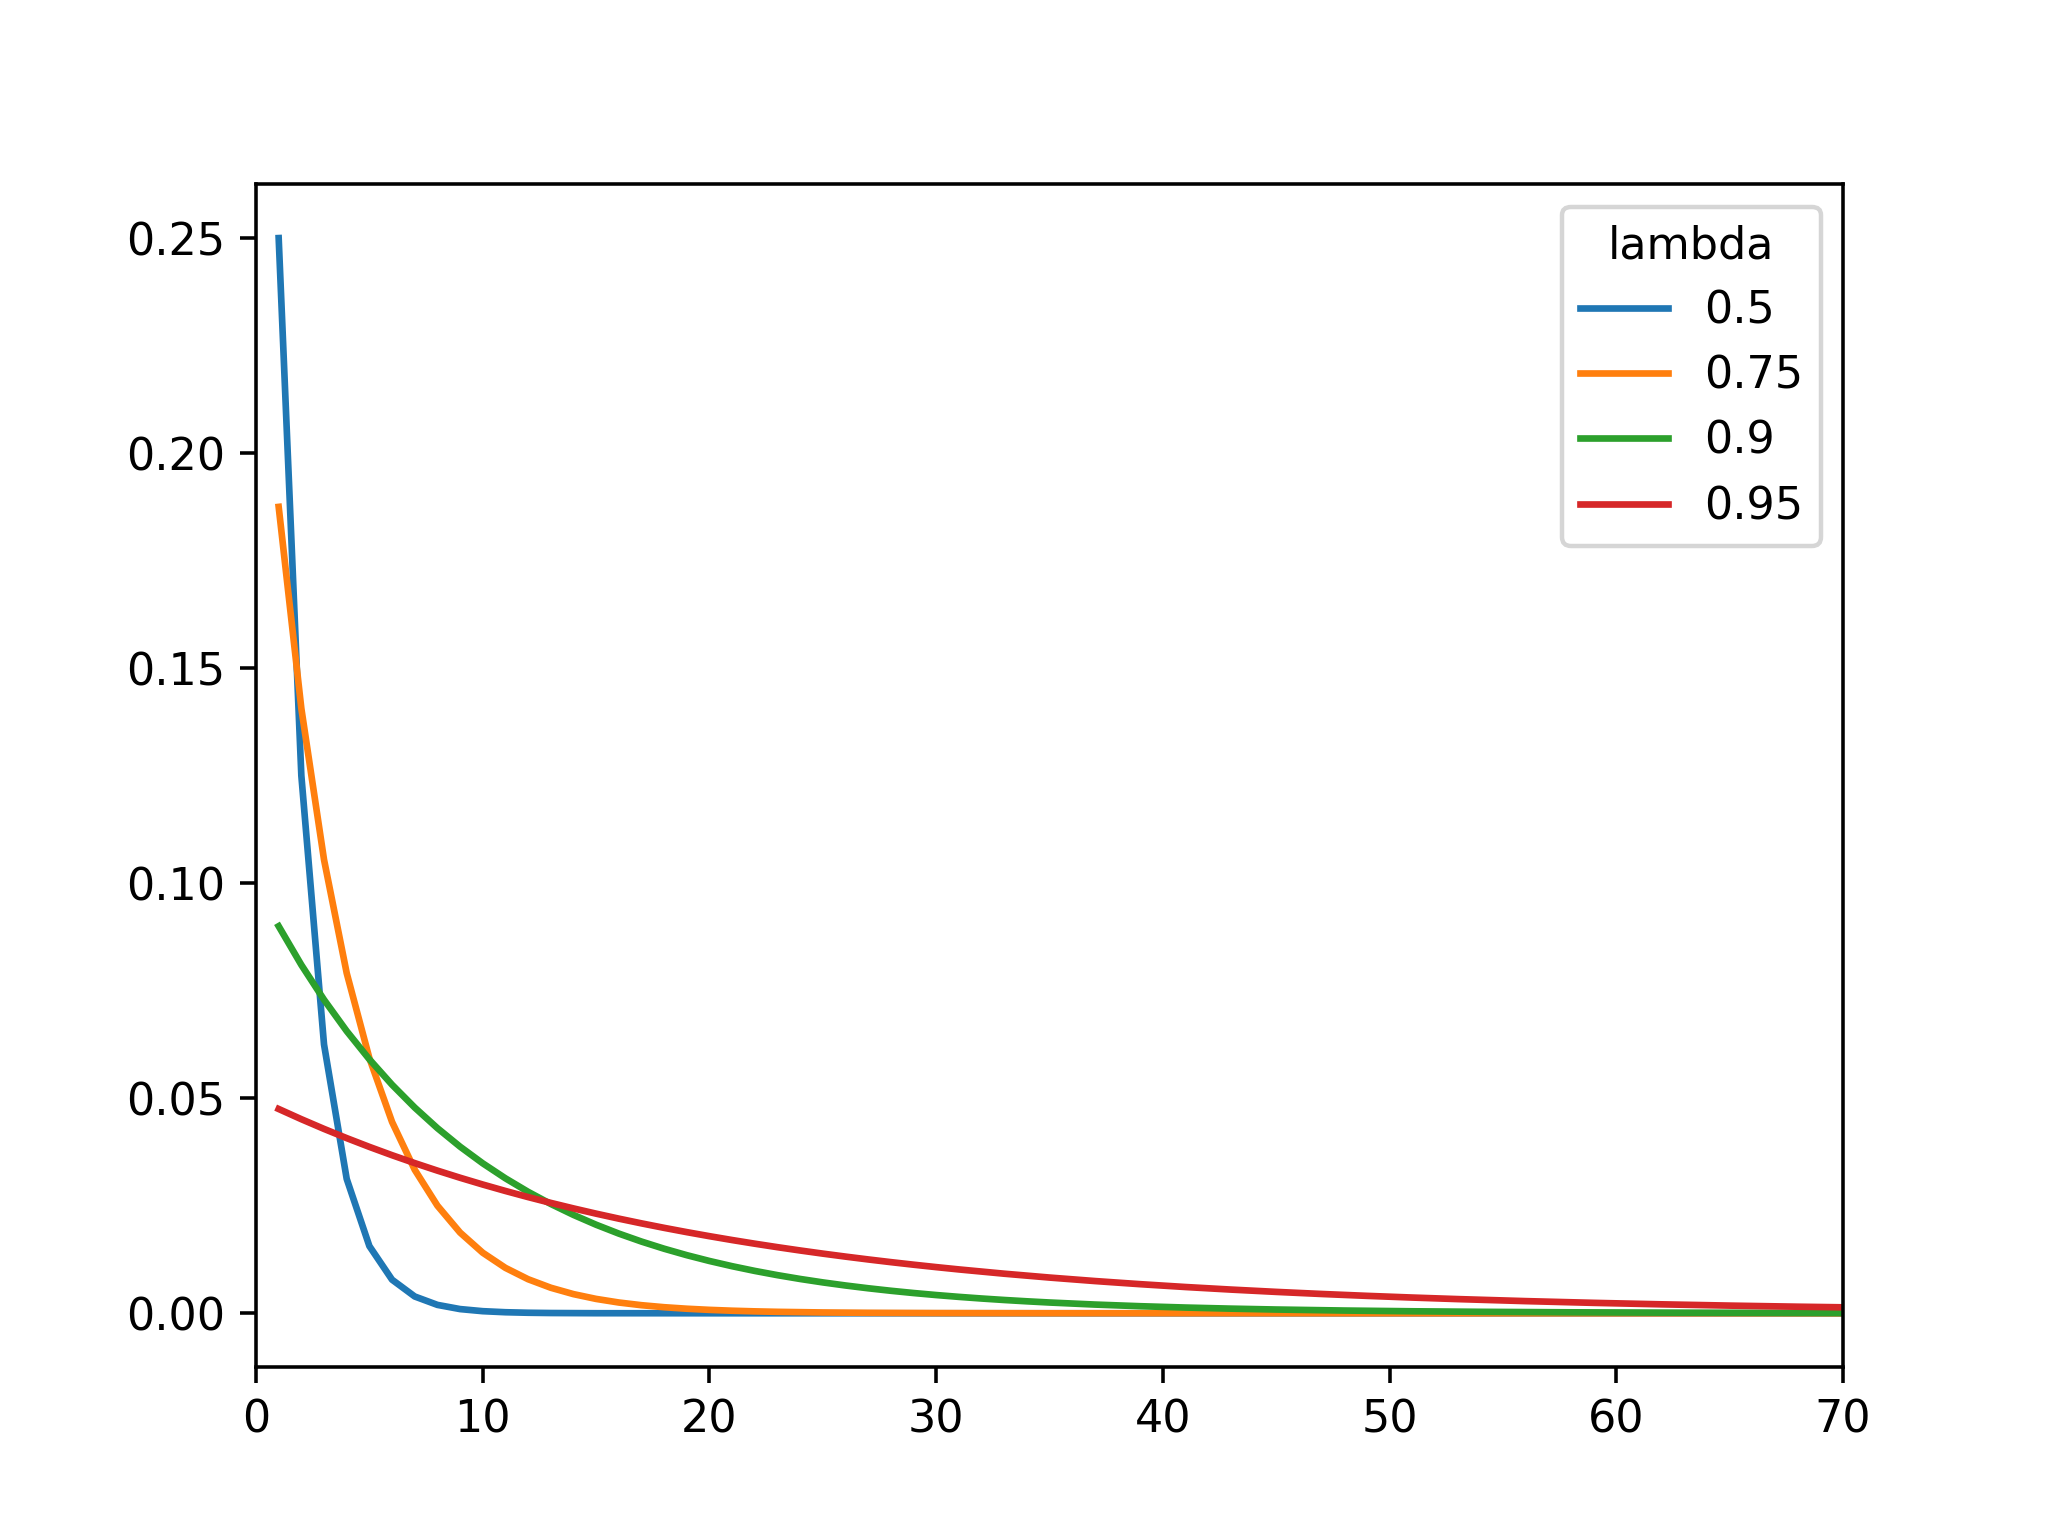
\includegraphics[width=0.75\textwidth]{images/lambda_return_weight.png}
    \caption{تاثیر پارامتر  $\lambda$ بر اهمیت پاداش‌های آینده. 
    محور افقی نماینده تعداد گام‌ها، و محور عمودی نماینده وزن این بازگشت متناظر با آن است.}\label{fig:td_lambda}
    
\end{figure}
\subsubsection{تی‌دی لامبدا رو به عقب}
در روش تی‌دی $\lambda$ با دید رو به عقب،
از مفهومی به نام آثار شایستگی\LTRfootnote{Eligibility Traces} استفاده می‌شود.
این مفهوم، نشان‌دهنده‌ی این است که هر عملی که در گذشته انجام شده و موجب تغییر ارزش عملی شده است،  به چه میزان روی این تغییر سهیم بوده‌است\cite{geist2014off}.

ابتدا به ازای هر حالت و عمل، یک متغیر آثار شایستگی $E(s, a)$
صفر تعیین می‌شود و سپس در هر گام، این متغیر به صورت زیر به‌روز‌رسانی می‌شود:
\begin{equation}\label{eq:eligibility_trace}
    E(s, a) = \gamma \times \lambda \times E(s, a) + 1(s = s_t, a = a_t)
\end{equation}
در واقع کل آثار شایستگی در لامبدا ضرب شده، و یکی به آثار شایستگی عمل و حالت فعلی اضافه می‌شود.
در این حالت، آثار شایستگی معادل با میزان نزدیکی زمانی هر حالت و عمل، به حالت و عمل فعلی است.

سپس ارزش عمل به صورت زیر به‌روز‌رسانی می‌شود:
\begin{equation}\label{eq:td_lambda_backward_q_function}
    Q(s, a) = Q(s, a) + \alpha \times \delta \times E(s, a)
\end{equation}
که در این رابطه، $\delta$
خطای تخمین\LTRfootnote{Estimate Error}
 است که به صورت زیر محاسبه می‌شود:
\begin{equation}\label{eq:td_lambda_backward_delta}
    \delta = R_{t+1} + \gamma \times (Q(s_{t+1}, a_{t+1}) - Q(s_t, a_t))
\end{equation}
می‌توان نشان داد که پس از انجام یک قسمت، به‌روز‌رسانی‌های انجام شده توسط این روش، معادل با به‌روز‌رسانی‌های انجام شده توسط تی‌دی $\lambda$ با دید رو به جلو است.

با ترکیب این روش و سیاست اپسیلون-حریصانه، می‌توان به یک روش یادگیری تقویتی کارا دست یافت که 
سارسا-لامبدا\LTRfootnote{SARSA($\lambda$)} نام دارد.
\section{استفاده از تقریب‌گر تابع}
با توجه به زیاد بودن تعداد حالت‌های ممکن در اکثر مسائل، یادگیری با روش‌های توضیح‌داده‌شده بسیار کند و حتی غیرمعقول می‌باشد\cite{kimura1997reinforcement}.
از این رو، به جای نگه‌داری مقادیر \lr{Q} 
در یک جدول به ازای هر زوج حالت-عمل
 از تقریب‌گر‌های تابع\LTRfootnote{Function Approximators}
  برای تخمین این مقادیر استفاده می‌کنیم.

    از تقریب‌گر‌های تابع مختلفی می‌توان برای این کار استفاده کرد.
    از جمله‌ی این تقریب‌گر‌ها می‌توان به شبکه‌های عصبی، درخت‌های تصمیم، و توابع پایه‌ای مثل چندجمله‌ای‌ها اشاره کرد.

    در واقع ابتدا از حالت، برخی ویژگی‌های مهم را استخراج کرده، سپس از این ویژگی‌ها برای تخمین ارزش‌ها به کمک پارامتر‌هایی که قرار است یاد گرفته شوند استفاده می‌کنیم.
    رایج است که در روابط، به این پارامتر‌ها با 
    $\theta$ یا $w$
    اشاره شود.

\begin{figure}[H]
    \centering
    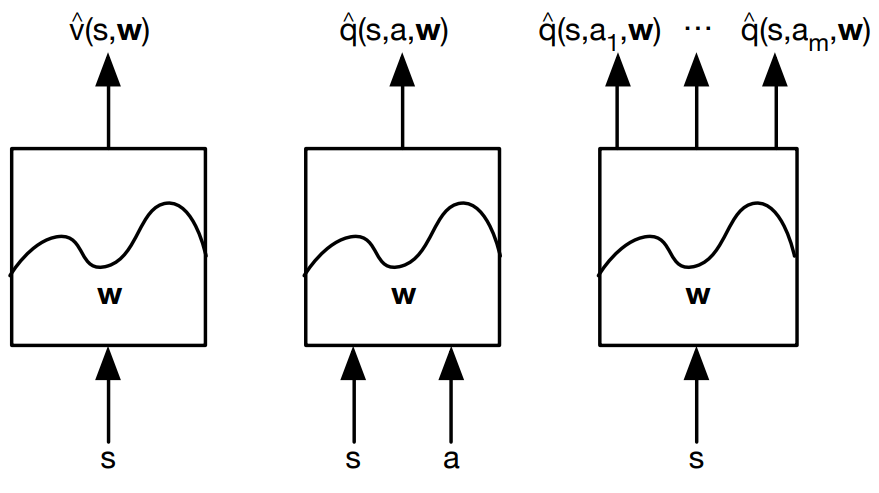
\includegraphics[width=0.75\textwidth]{images/function_approximators.png}
    \caption{روش‌های مختلف استفاده از تقریب‌گر تابع}\label{fig:func_approx}
\end{figure}
حال کافی‌ست که معادلات \ref{eq:td_zero_q_function}، \ref{eq:td_lambda_q_function}، و \ref{eq:td_lambda_backward_q_function} را به صورت تقریبی برای تقریب‌گر تابع بنویسیم
و به‌جای به‌روز‌رسانی مقادیر \lr{Q}، پارامتر‌های تقریب‌گر تابع را به‌روز کنیم.
با توجه به نیاز به به‌روز‌رسانی، لازم است از تقریب‌گر‌های مشتق‌پذیر استفاده کنیم.
همانطور که در عکس \ref{fig:func_approx}
می‌توان دید، در حالتی که از تقریب‌گر‌های تابع برای پیش‌بینی مقادیر \lr{Q} استفاده می‌شود،
رایج است از عبارت 
$Q(s, a; \theta)$
یا $Q(s, a; w)$
برای نشان دادن این تقریب‌گر‌ها استفاده کرد.

\section{الگوریتم شبکه کیو عمیق}
الگوریتم شبکه کیو عمیق\LTRfootnote{Deep Q Network (DQN)}
 یکی از مستقیم‌ترین راه‌های استفاده از تقریب‌گر‌های توابع برای ترکیب یادگیری عمیق و تقویتی است.
در این الگوریتم، هدف این است که مشابه با حالت سوم شکل \ref{fig:func_approx}،
پارامتر‌های یک شبکه عصبی را به‌گونه‌ای تنظیم کنیم که مقادیر ارزش عمل را بتواند تخمین بزند.
از دستاورد‌های این الگوریتم، عملکرد در حد انسان در چندین بازی آتاری\LTRfootnote{Atari} است
که توسط تیم دیپ‌مایند\LTRfootnote{DeepMind}
در سال ۲۰۱۵ به‌وقوع پیوست\cite{mnih2013playing}.

شبکه‌های عصبی الهام گرفته از ساختار و عملکرد مغز انسان هستند که برای یادگیری از داده‌ها و تصمیم‌گیری‌های پیچیده استفاده می‌شوند.
 این شبکه‌ها از واحدهای پردازشی به نام پرسپترون‌ها\LTRfootnote{Perceptrons}
  تشکیل شده‌اند که در لایه‌های مختلف قرار گرفته‌اند و از طریق وزن‌هایی به هم متصل می‌شوند.
 
 یادگیری در شبکه‌های عصبی اغلب از طریق فرایندی به نام نزول گرادیان\LTRfootnote{Gradient Descent}
  انجام می‌گیرد که در آن وزن‌های شبکه به صورت مکرر تنظیم می‌شوند تا خطا بین پیش‌بینی‌های شبکه و داده‌های واقعی به حداقل برسد. این فرایند شامل محاسبه گرادیان یا شیب تابع خطا نسبت به وزن‌ها و به‌روزرسانی وزن‌ها در جهت مخالف گرادیان برای کاهش خطا است.
% formula for gradient descent
\begin{equation}\label{eq:gradient_descent}
    \theta_{t+1} = \theta_t - \alpha \nabla J(\theta_t)
\end{equation}
در این فرمول، $\theta$
پارامتر‌های شبکه،
\lr{$\alpha$}
نرخ یادگیری،
\lr{$J$}
تابع خطا، و
\lr{$\nabla J$}
گرادیان تابع خطا نسبت به پارامتر‌ها هستند.

برای اینکه یادگیری شبکه عصبی با ثبات بالاتری رخ دهد، این الگوریتم از دو تکنیک 
\textbf{بازیابی تجربه}\LTRfootnote{Experience Replay}\cite{fedus2020revisiting}
و
\textbf{استفاده از شبکه هدف}\LTRfootnote{Target Network}
بهره می‌برد.
\subsection{بازیابی تجربه}
برای رفع مشکلات داده‌های همبسته و توزیع‌های غیر ایستا در یادگیری برخط، \lr{DQN} از یک مکانیزم بازیابی تجربه استفاده می‌کند. این شامل ذخیره تجربیات عامل در هر گام زمانی در یک بافر بازیابی و سپس نمونه‌برداری تصادفی ریزدسته‌ها\LTRfootnote{Mini-batches}
 از این بافر برای آموزش شبکه است. این رویکرد به شکستن همبستگی بین نمونه‌های پیاپی کمک می‌کند و فرآیند یادگیری را پایدار می‌سازد.
\subsection{استفاده از شبکه هدف}
\lr{DQN}
 یک شبکه دوم به نام شبکه هدف را برای استقرار بیشتر آموزش معرفی می‌کند. شبکه هدف یک کپی از شبکه 
 \lr{Q}
  است؛ اما وزن‌های آن با بسامد کمتری به‌روز می‌شوند. این جداسازی نوسان ارزش‌های هدف در به‌روزرسانی یادگیری 
  \lr{Q}
   را کاهش می‌دهد و خطر حلقه‌های بازخورد خودتقویتی\LTRfootnote{Self-Reinforced Feedback Loop}
    را کاهش می‌دهد.
\subsection{فرآیند یادگیری}
در ابتدا وزن‌های شبکه ارزش عمل را به صورت تصادفی تنظیم می‌کنیم و آن را $\theta$ می‌نامیم.
 شبکه هدف را با وزن‌های یکسان مقداردهی می‌کنیم و آن را $\theta^-$ می‌نامیم.
و بافر بازیابی را
به طول $N$ که یک ابرپارامتر\LTRfootnote{Hyperparameter}
 است، مقداردهی می‌کنیم.

سپس در هر حالت، پاداش‌های خروجی شبکه اصلی را می‌گیریم و به صورت اپسیلون-حریصانه عمل را انتخاب می‌کنیم؛
یعنی به احتمال $\epsilon$ رفتار تصادفی داریم، 
و با احتمال $1-\epsilon$
رفتار با بالاترین ارزش عمل پیش‌بینی شده را برمیداریم، به عبارتی: $a_t = \underset{a}{\mathrm{argmax}} Q(s_t, a; \theta)$.

ترکیب چهارتایی حالت قبل عمل، عمل انتخاب شده، پاداش دریافتی، و حالت بعد عمل $(s_t,a_t,r_t,s_{t+1})$
را به بافر اضافه می‌کنیم.
یک گروه با اندازه مشخص را با نمونه‌برداری تصادفی از بافر انتخاب می‌کنیم، و به صورت زیر یادگیری را انجام می‌دهیم:
\begin{equation}\label{dqn_label}
    y_j = \begin{cases}
        r_j & \text{اگر $s_{j+1}$ حالت پایانی قسمت باشد} \\
        r_j + \gamma \times \max_{a'} Q(s_{j+1}, a'; \theta^-) & \text{در غیر این صورت}
    \end{cases}
\end{equation}
در این معادله $y_j$ تخمینی از میزان پاداش دریافتی واقعی است، که مشابه با روش‌های تفاوت زمانی، از ترکیب پاداش دریافتی و ارزش عمل بعدی به دست می‌آید.
بنابرین می‌توان از این مقدار، مشابه با برچسب در یادگیری نظارت‌شده، برای آموزش شبکه استفاده کرد.
میزان خطای شبکه به صورت زیر تعریف می‌شود:
\begin{equation}\label{dqn_loss}
    L(\theta) = \mathbb{E}[(y_j - Q(s_j, a_j; \theta))^2]
\end{equation}
که با استفاده از این خطا، می‌توان گرادیان تابع خطا نسبت به وزن‌های شبکه را به دست آورد و
با استفاده از این گرادیان، می‌توان وزن‌های شبکه را به‌روز کرد:
\begin{equation}\label{dqn_update}
    \theta_{t+1} = \theta_t - \alpha \nabla_\theta L(\theta)
\end{equation}
در نهایت کافی‌ست به صورت تناوبی و هر چند گام یک بار وزن‌های شبکه هدف را برابر با کپی وزن‌های شبکه اصلی قرار دهیم. با تکرار این مراحل، به شبکه عصبی‌ای دست می‌یابیم که قدرت پیش‌بینی ارزش‌های عمل را دارد.


حال می‌توان اهمیت دو تکنیک گفته شده را بهتر فهمید: در صورت عدم استفاده از شبکه هدف، باید همزمان از شبکه اصلی برای پیش‌بینی آینده (در فرمول \ref{dqn_label}) و انتخاب عمل استفاده کنیم، که می‌تواند به مشکلاتی مانند نوسانات در آموزش و حلقه‌های بازخورد خودتقویتی منجر شود.
همچنین در صورت عدم استفاده از بافر تجربه، باید صرفا از تجارب اخیر خود استفاده کنیم، که در این صورت همبستگی بین نمونه‌ها و توزیع‌های غیر ایستا می‌تواند مشکل‌ساز شود.

در بسیاری از پیاده‌سازی‌ها، مقدار اپسیلون که به آن نرخ کاوش\LTRfootnote{Exploration Rate}
 هم گفته می‌شود، متغیر است و ابتدا زیاد بوده و در طول آموزش به تدریج کاهش می‌یابد و به مقدار ثابتی می‌رسد.
\subsection{اثرات برخی از ابرپارامتر‌ها}
در این بخش به بررسی تاثیر تغییر «اندازه ریزدسته» و «اندازه بافر تجربه» بر عملکرد الگوریتم \lr{DQN} می‌پردازیم.
\subsubsection{اندازه ریزدسته}
اندازه ریزدسته تعداد نمونه‌هایی است که از بافر تجربه برای آموزش شبکه استفاده می‌شود.
با افزایش این مقدار، تنوع نمونه‌ها افزایش می‌یابد و از طرف دیگر، باعث افزایش پیچیدگی محاسباتی می‌شود.
بنابرین باید یک تعادل بین زمان لازم برای هر به‌روز‌رسانی شبکه، و کیفیت آموزش شبکه داشته باشیم.
\subsubsection{اندازه بافر تجربه}
اندازه بافر تجربه تعداد نمونه‌هایی است که برای آموزش شبکه در طول یادگیری ذخیره می‌شود.
با افزایش این تعداد، تنوع این تجربه‌ها افزایش می‌یابد و از طرف دیگر، باعث افزایش حافظه مصرفی می‌شود.

در صورت زیادی کوچک بودن این پارامتر، فقط تجارب اخیر در بافر ذخیره می‌شوند و از تجربیات گذشته استفاده نمی‌شود.
بنابرین عامل ممکن است فراموشی تجربیات گذشته را تجربه کند و یادگیری برخط آن را مختل کند\cite{zhang2017deeper}.
از سوی دیگر، در صورت کوچک بودن تجربیات، احتمال وجود تجارب اخیر درون ریزدسته کاهش می‌یابد که باعث کند شدن فرآیند آموزش و عدم دریافت واکنش نسبت به امتحان کردن حالت‌های جدید می‌شود\cite{mnih2015human}.
بنابرین باید اندازه بافر نسبت به اندازه ریزدسته و همچنین طول کل آموزش به درستی انتخاب شود.  
\section{الگوریتم بهبود گرادیان سیاست معین عمیق}
الگوریتم بهبود گرادیان سیاست معین عمیق\LTRfootnote{Deep Deterministic Policy Gradient (DDPG)} یا به اختصار \lr{DDPG}، یک الگوریتم یادگیری تقویتی است که برای حل مسائل پیوسته و فضای عمل پیوسته طراحی شده است\cite{lillicrap2015continuous}.
همانطور که در بخش‌های قبل مشاهده کردیم، برای انتخاب عمل معمولا از سیاست اپسیلون-حریصانه استفاده می‌شود؛ اما این روش برای فضای عمل پیوسته مناسب نیست، چرا که به‌دست‌آوردن بیشینه در فضای پیوسته به مراتب دشوار‌تر از حالت گسسته است.
این الگوریتم از نوع یادگیری خارج از سیاست است؛ به این معنا که عامل با دنبال کردن سیاستی که سیاست انتخابی خود نیست به بهبود عملکرد خود می‌پردازد.

\lr{DDPG}
از دو شبکه عصبی استفاده می‌کند\cite{silver2014deterministic}: یک شبکه برای تخمین ارزش عمل که به آن نقاد\LTRfootnote{Critic}
 می‌گوییم، و یک شبکه برای تخمین سیاست و انتخاب عمل که به آن بازیگر\LTRfootnote{Actor}
  می‌گوییم.
شبکه نقاد مشابه با شبکه
 \lr{Q}
  در 
  \lr{DQN}
   است؛ با این تفاوت که حالت و عمل را ورودی گرفته و ارزش عمل را خروجی می‌دهد.
  شبکه سیاست یک شبکه عصبی است که خروجی آن عمل است.
 این الگوریتم مشابه با \lr{DQN}
 از بافر تجربه برای ذخیره تجربیات عامل، و از شبکه‌های هدف برای هر دو شبکه نقاد و بازیگر استفاده می‌کند.
 البته در این الگوریتم، به‌جای کپی وزن‌های شبکه به شبکه هدف، از میانگین وزن‌دار استفاده می‌شود تا به‌روز‌رسانی آرام‌تر انجام شود و ثبات بیشتری داشته باشد.
 \begin{figure}[H]
    \centering
    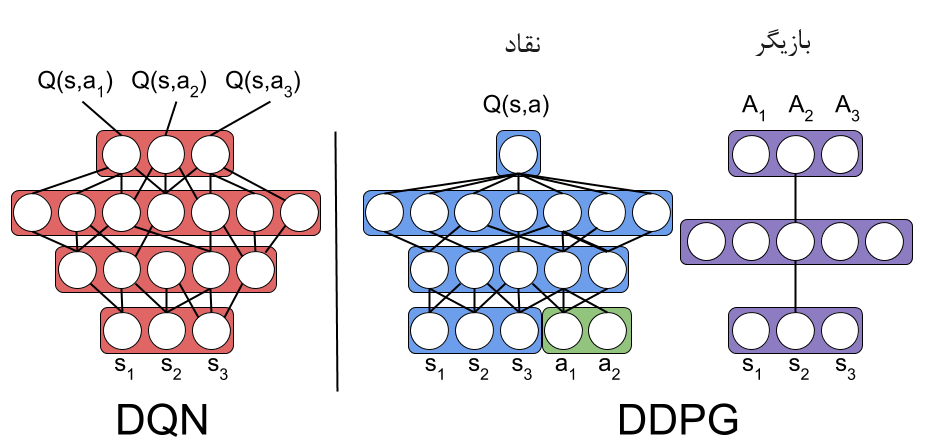
\includegraphics[width=0.85\textwidth]{images/actor_critic.png}
    \caption{شبکه‌های عصبی بازیگر و نقاد در الگوریتم \lr{DDPG} و مقایسه با \lr{DQN}}\label{fig:actor_critic}
\end{figure}
رایج است که شبکه ارزش عمل را با $Q(s, a; \phi)$ و شبکه سیاست را با $\mu(s; \theta)$ نشان دهیم.
فرآیند یادگیری این الگوریتم به صورت زیر است:
\begin{enumerate}
    \item ابتدا وزن‌های شبکه‌های نقاد و بازیگر را به صورت تصادفی مقداردهی می‌کنیم و آن‌ها را به ترتیب $\phi$ و $\theta$ می‌نامیم.
    \item بافر تجربه را به طول $N$ مقداردهی می‌کنیم.
    \item در هر گام زمانی، حالت را به شبکه بازیگر می‌دهیم و عملی که این شبکه پیشنهاد می‌دهد را انجام می‌دهیم.
    \item پاداش دریافتی و حالت بعد عمل را به بافر تجربه اضافه می‌کنیم.
    \item یک ریزدسته از بافر تجربه را انتخاب کرده و با استفاده از فرمول زیر، مقدار واقعی ارزش حالت را (طبق الگوریتم تفاوت زمانی) محاسبه می‌کنیم:
    \begin{equation}\label{ddpg_label}
        y_j = \begin{cases}
            r_j & \text{اگر $s_{j+1}$ حالت پایانی قسمت باشد} \\
            r_j + \gamma \times Q(s_{j+1}, \mu(s_{j+1}; \theta^-); \phi^-) & \text{در غیر این صورت}
        \end{cases}
    \end{equation}
    \item خطای شبکه نقاد را به صورت زیر محاسبه می‌کنیم:
    \begin{equation}\label{ddpg_critic_loss}
        L(\phi) = \mathbb{E}[(y_j - Q(s_j, a_j; \phi))^2]
    \end{equation}
    و وزن‌های شبکه نقاد را به‌روز می‌کنیم:
    \begin{equation}\label{ddpg_critic_update}
        \phi_{t+1} = \phi_t - \alpha \nabla_\phi L(\phi)
    \end{equation}
    \item خطای شبکه بازیگر را به صورت زیر محاسبه می‌کنیم:
    \begin{equation}\label{ddpg_actor_loss}
        L(\theta) = -\mathbb{E}[Q(s, \mu(s; \theta); \phi)]
    \end{equation}
    و وزن‌های شبکه بازیگر را به‌روز می‌کنیم:
    \begin{equation}\label{ddpg_actor_update}
        \theta_{t+1} = \theta_t + \alpha \nabla_\theta L(\theta)
    \end{equation}
    \item در نهایت هر چند گام یک بار، وزن‌های شبکه‌های هدف را به‌روز می‌کنیم:
    \begin{equation}\label{ddpg_target_actor_update}
        \theta^-_{t+1} = \tau \theta_t + (1-\tau) \theta^-_t
    \end{equation}
    \begin{equation}\label{ddpg_target_critic_update}
        \phi^-_{t+1} = \tau \phi_t + (1-\tau) \phi^-_t
    \end{equation}
\end{enumerate}
همانطور که مشاهده‌شد، این الگوریتم تعداد زیادی ابرپارامتر دارد که باید به درستی تنظیم شوند تا به عملکرد بهینه برسد.
از جمله این پارامتر‌ها می‌توان به نرخ یادگیری ($\alpha$ که می‌تواند برای شبکه‌های نقاد و بازیگر متفاوت باشد)،
، نرخ تخفیف ($\gamma$)،
فرکانس به‌روزرسانی شبکه‌ها (هر چند گام یک بار ریزدسته انتخاب می‌کنیم و مراحل ۵ تا ۸ را طی می‌کنیم)،
فرکانس به‌روزرسانی وزن‌های هدف (هر چند گام یک بار وزن‌های شبکه‌های هدف را به‌روزرسانی می‌کنیم)
 ، اندازه ریزدسته، طول بافر تجربه، و ضریب میانگین‌گیری برای به‌روزرسانی شبکه‌های هدف ($\tau$)
  اشاره کرد.
\section{جمع‌بندی}
در این فصل، ابتدا به معنا و اهمیت یادگیری تقویتی پرداختیم و سپس به معرفی مفاهیم اصلی این حوزه پرداختیم.
سپس به معرفی الگوریتم‌های یادگیری تقویتی کلاسیک بر مبنای مدل همچون برنامه‌نویسی پویا و روش‌های مبتنی بر ارزش و سیاست پرداختیم.
در ادامه به معرفی الگوریتم‌های یادگیری تقویتی بدون مدل پرداختیم که از تقریب‌گر‌های تابع برای تخمین ارزش‌ها استفاده می‌کنند.
در این بخش، به معرفی دو الگوریتم معروف یادگیری تقویتی بدون مدل، یعنی \lr{DQN} و \lr{DDPG} پرداختیم.
در ادامه، در فصل بعد به معرفی یک مسئله و کاربرد این الگوریتم‌ها در حل آن خواهیم پرداخت.
